\section{Kinematics}
\subsection{Vector notation}
There are two ways of expressing vectors:
\begin{subequations}
\begin{align}
    \mathbf{r}^i &= \begin{bmatrix} a \\ b \\ c \end{bmatrix} \\
    \vec{r}_{a/b} &= a\vec{i}_i + b\vec{j}_i + c\vec{k}_i
\end{align}
\end{subequations}
Where $i$ is the frame of reference, and subscript $a/b$ denotes from point b to point a. If the vectors are velocities, subscript $a/b$ denotes the velocity of point a relative to point b.
It is important to be consistent in the notation. Never do arithmetic operations on vectors expressed in different frames. This means: \newline
\begin{subequations}
\begin{align}
    \bcancel{\cancel{\vec{r}^i}}\\
    \bcancel{\cancel{\mathbf{v}^i+\mathbf{u}^a}}\\
    \bcancel{\cancel{\mathbf{v}^i \times \mathbf{u}^a}}
\end{align}
\end{subequations}

\subsection{Skew matrix notation}
If you have $\mathbf{u} = \begin{bmatrix}u_1 & u_2 & u_3\end{bmatrix}^\top$ and $\mathbf{v} = \begin{bmatrix}v_1 & v_2 & v_3\end{bmatrix}^\top$:
\begin{subequations}
    \begin{align}
    \mathbf{u}^\times = \begin{bmatrix}
                    0 & -u_3 & u_2 \\
                    u_3 & 0 & -u_1 \\
                    -u_2 & u_1 & 0
                  \end{bmatrix} \\
    \mathbf{u}^\times \mathbf{v} = \mathbf{u} \times \mathbf{v} \\
    \mathbf{u}^\times \mathbf{u} = 0 \\
    \left(\mathbf{u}^\times\right)^\times = -\mathbf{u}^\times \\
    \det{(\mathbf{u}^\times)} = 0  
    \end{align}
\end{subequations}
The cross product of two vectors can be calculated by finding the determinant of this matrix:
\begin{equation}
    \mathbf{u} \times \mathbf{v} = \det{\begin{bmatrix}
                    \vec{i} & \vec{j} & \vec{k} \\
                    u_1 & u_2 & u_3 \\
                    v_1 & v_2 & v_3
                  \end{bmatrix}}
\end{equation}

\subsection{Rotation matrices}
The rotation matrices are defined on each axis as:
\begin{subequations}
    \begin{align}
    \mathbf{R}_x(\theta) &= \begin{bmatrix} 1 & 0 & 0 \\ 0 & \cos(\theta) & -\sin(\theta) \\ 0 & \sin(\theta) & \cos(\theta) \end{bmatrix} \\
    \mathbf{R}_y(\phi) &= \begin{bmatrix} \cos(\phi) & 0 & \sin(\phi) \\ 0 & 1 & 0 \\ -\sin(\phi) & 0 & \cos(\phi) \end{bmatrix} \\
    \mathbf{R}_z(\psi) &= \begin{bmatrix} \cos(\psi) & -\sin(\psi) & 0 \\ \sin(\psi) & \cos(\psi) & 0 \\ 0 & 0 & 1 \end{bmatrix}
    \end{align}
\end{subequations}
Now lets say frame $a$ relative to frame $i$ is rotated by $\theta$ about the $x$-axis, $\phi$ about the $y$-axis, and $\psi$ about the $z$-axis. The rotation matrix from frame $a$ to frame $i$ is then:
\begin{equation}
    \mathbf{R}_i^a = \mathbf{R}_z(\psi)\mathbf{R}_y(\phi)\mathbf{R}_x(\theta)
\end{equation}
Which means that $\mathbf{R}_i^a$ is called the \textit{rotation matrix} from frame $a$ to frame $i$. Visually this is seen as moving the referance frame from $a$ to $i$, but it is used in transforming a vector from $i$ to $a$ (THE OPPOSITE ARG) for example: 
\begin{equation}
    \mathbf{v}_b = \mathbf{R}_i^b\mathbf{v}_i
\end{equation}
\begin{figure}[H]
    \centering
    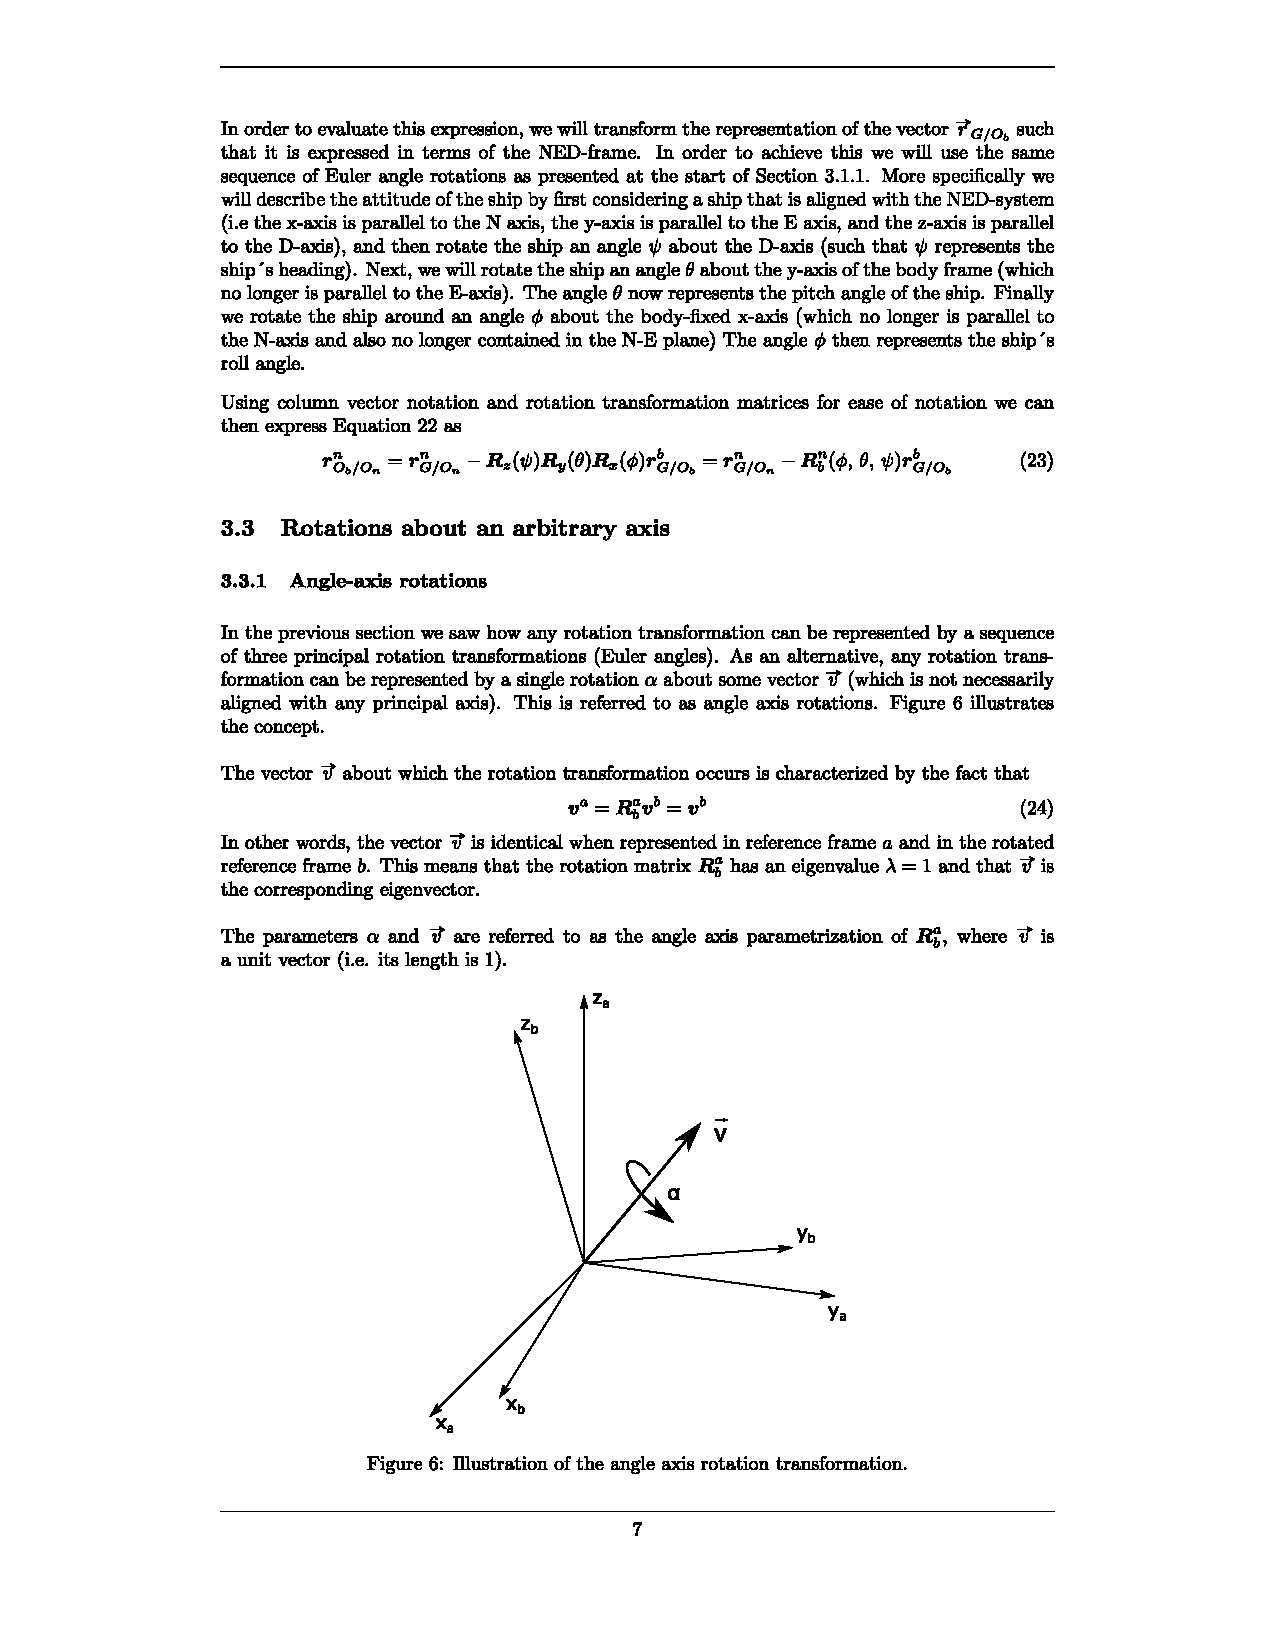
\includegraphics[scale=1, trim={7cm 3.5cm 7cm 16.5cm}, clip]{figures/arbitrary_axis_rotation.pdf}
    \caption{Rotation about arbitrary axis}
    \label{fig:arbitrary_axis_rotation}
\end{figure}
Now, if we have a rotation about an arbitrary axis $\mathbf{v}$, we can use the equation:
\begin{equation}
    \mathbf{R}_{\alpha,\vec{v}} = \cos(\alpha)\mathbf{I} + \mathbf{v}^\times\sin(\alpha) + \mathbf{vv}^\top(1-\cos(\alpha)) = \mathbf{R}_b^a(\alpha)
\end{equation}
\subsubsection{Properties of rotation matrices}
A couple of maybe interesting properties of rotation matrices:
\begin{subequations}
    \begin{align}
        \mathbf{v}^b=\mathbf{R}_a^b\mathbf{v}^a \\
        \mathbf{v}^a=\mathbf{R}_b^a\mathbf{v}^b \\
        \mathbf{R}_a^b\mathbf{R}_b^a = \mathbf{I} \\
        \mathbf{R}_a^b = \left(\mathbf{R}_b^a\right)^{-1} = \left(\mathbf{R}_b^a\right)^\top \\
        \dot{\mathbf{R}}_b^a = \left(\mathbf{\omega}_{ab}^a\right)^\times\mathbf{R}_b^a = \mathbf{R}_b^a\left(\mathbf{\omega}_{ab}^b\right)^\times \\
        \left(\vec{\omega}_{ab}^a\right)^\times = \dot{\mathbf{R}}_b^a\left(\mathbf{R}_b^a\right)^\top \\
        \vec{\omega}_{ad} = \vec{\omega}_{ab} + \vec{\omega}_{bc} + \vec{\omega}_{cd}
    \end{align}
\end{subequations}
Where the vector $\vec{\omega}_{ab}^a$ is the angular velocity vector from frame \textit{b} relative to frame \textit{b} with respect to frame \textit{a}.

\subsection{Linear and Angular Velocities and Acceleration in Different Frames}

Let \( \{0\} \) be the reference frame with coordinates \( x_0, y_0, z_0 \) and \( \{b\} \) be the body frame with coordinates \( x_b, y_b, z_b \). 

\subsection{Linear Velocity}

The linear velocity \( \vec{v}_{p/0} \) of a point \( p \) in the body frame \( \{b\} \) relative to the reference frame \( \{0\} \) is given by:

\[
\vec{v}_{p/0} = \vec{v}_0 + \vec{\omega}_{b/0} \times \vec{r}_{p/b}
\]

where:
\begin{itemize}
    \item \( \vec{v}_{p/0} \) is the linear velocity of point \( p \) in frame \( \{b\} \) relative to frame \( \{0\} \).
    \item \( \vec{v}_0 \) is the linear velocity of the origin of frame.
    \item \( \vec{\omega}_{b/0} \) is the angular velocity of frame \( \{b\} \) relative to frame \( \{0\} \).
    \item \( \vec{r}_{p/b} \) is the position vector of point p relative to the body frame \( \{b\} \).
\end{itemize}

\subsection{Linear Velocity with Time-Dependent Point \( p \)}

If the point \( p \) is a function of time, the linear velocity \( \vec{v}_{p/0} \) of a point \( p \) in the body frame \( \{b\} \) relative to the reference frame \( \{0\} \) is given by:

\[
\vec{v}_{p/0} = \vec{v}_{b/0} + \vec{\omega}_{b/0} \times \vec{r}_{p/b} + \vec{v}_{p/b}
\]

where \( \vec{v}_{p/b} \) is the velocity of point \( p \) relative to the body frame \( \{b\} \), given by:

\[
\vec{v}_{p/b} = \dot{p}_x \vec{i}_b + \dot{p}_y \vec{j}_b + \dot{p}_z \vec{k}_b
\]

Here, \( \dot{p}_x, \dot{p}_y, \dot{p}_z \) are the time derivatives of the coordinates of point \( p \) in the body frame.
    
\end{itemize}
\begin{itemize}
    \item \textbf{Alternative approach}
    This can also just be found by finding a the function for the point p in the zero frame ie:  (\( \vec{r}_{p/0} \)) and derivating this with respect to time. Remebering the importance of the chain rule this becomes equivalent and easy to solve on a beast calculator. (contact 41401071 for good price on beast calculator)
\end{itemize}


\subsection{Angular Velocity}

The angular velocity \( \vec{\omega}_{p} \) of point \( p \) is given by the sum of all contributing angular velocities:

\[
\vec{\omega_{p}} = \sum_{i} \omega_i \vec{e}_i
\]

where \( \omega_i \) are the individual angular velocity components about their respective principal axes \( \vec{e}_i \), representing the axis of rotation (it could be along $x_b$, $y_b$, or $z_b$).

\subsection{Angular Acceleration}

The angular acceleration \( \vec{\alpha}_{p} \) of point \( p \) is given by:

\[
\vec{\alpha_{p}} = \sum_{i} \dot{\omega}_i \vec{e}_i + \omega_i (\vec{\Omega}_i \times \vec{e}_i)
\]

where:
\begin{itemize}
    \item \( \dot{\omega}_i \) is the time derivative of the angular velocity component \( \omega_i \).
    \item \( \vec{\Omega}_i \) is the angular velocity of the reference frame of \( \mathbf{e}_i \).
    \item \( \vec{e}_i \) are the principal axes of the reference frame.
\end{itemize}

\subsection{Linear Acceleration}

The linear acceleration \( \vec{a}_{p/0} \) of point \( p \) relative to the reference frame \( \{0\} \) is given by:

\[
\vec{a}_{p/0} = \vec{a}_{b/0} + \vec{a}_{p/b} + \vec{\alpha}_{b/0} \times \vec{r}_{p/b} + \vec{\omega}_{b/0} \times (\vec{\omega}_{b/0} \times \vec{r}_{p/b}) + 2 \vec{\omega}_{b/0} \times \vec{v}_{p/b}
\]

where:
\begin{itemize}
    \item \( \vec{a}_{b/0} \) is the acceleration of the origin of the body frame \( \{b\} \) relative to the reference frame \( \{0\} \).
    \item \( \vec{a}_{p/b} \) is the acceleration of point \( p \) relative to the body frame \( \{b\} \).
    \item \( \vec{\alpha}_{b/0} \) is the angular acceleration of the body frame \( \{b\} \) relative to the reference frame \( \{0\} \).
    \item \( \vec{\omega}_{b/0} \) is the angular velocity of the body frame \( \{b\} \) relative to the reference frame \( \{0\} \).
    \item \( \vec{r}_{p/b} \) is the position vector of point p relative to the body frame \( \{b\} \).
\end{itemize}

\subsection{Explanation of Acceleration Components}

\begin{itemize}
    \item \textbf{Acceleration of Origin of Body Frame} (\( \vec{a}_{b/0} \)): This term represents the linear acceleration of the origin of the body frame \( \{b\} \) relative to the reference frame \( \{0\} \).
    \item \textbf{Acceleration of Point within Body Frame} (\( \vec{a}_{p/b} \)): This term represents the linear acceleration of point \( p \) within the body frame \( \{b\} \).
    \item \textbf{Linear Acceleration due to Angular Acceleration} (\( \vec{\alpha}_{b/0} \times \vec{r}_{p/b} \)): This term accounts for the linear acceleration of point \( p \) due to the angular acceleration of the body frame \( \{b\} \).
    \item \textbf{Centripetal Acceleration} (\( \vec{\omega}_{b/0} \times (\vec{\omega}_{b/0} \times \vec{r}_{p/b}) \)): This term represents the centripetal acceleration, which is the acceleration of point \( p \) due to its rotational motion about the origin of the body frame \( \{b\} \).
    \item \textbf{Coriolis Acceleration} (\( 2 \vec{\omega}_{b/0} \times \vec{v}_{p/b} \)): This term represents the Coriolis acceleration, which arises when point \( p \) is moving within the rotating body frame \( \{b\} \).
\end{itemize}



\subsection{Other stuff that might be usefull}
\textbf{Linear momentum} does not depend upn its point of reference:
\begin{subequations}
    \begin{align}
        \vec{p} = m\vec{v} \\
        \dot{\vec{p}} = m\vec{a} = \vec{F}
    \end{align}
\end{subequations}
\textbf{Angular momentum} of point \textit{p} with respect t origin \textit{o}, where $\vec{r}_{p/o}$ is the position of \textit{p} and $\vec{p}$ is the linear momentum. (Angular momentum depends upon its point of reference):
\begin{subequations}
    \begin{align}
        \vec{h}_{p/o} = \vec{r}_{p/o} \times \vec{p} \\
        \dot{\vec{h}}_{p/o} = \vec{r}_{p/o} \times \dot{\vec{p}} = \vec{T}
    \end{align}
\end{subequations}